\documentclass[a4paper]{article}

\usepackage[portuguese]{babel}
\usepackage[utf8]{inputenc}
\usepackage[T1]{fontenc}

\newcommand{\documentTitle}{Photorealistic Graphics - Photon mapping} %Macro definition
\newcommand{\documentAuthors}{João Rafael (2008111876, jprafael@student.dei.uc.pt) \and José Ribeiro (2008112181, jbaia@student.dei.uc.pt)} %Macro definition

\title{\documentTitle}
\author{\documentAuthors{}}

\usepackage{hyperref}
\hypersetup{
	pdftitle = \documentTitle
	,pdfauthor = \documentAuthors
	,pdfsubject = {Computer Graphics Project \#2 Report}
	,pdfkeywords = {Computer Graphics Project} {Photon Mapping} {Raytracing}
	,pdfborder = {0 0 0}
}

\usepackage{subfig}
\usepackage{amsmath}
\usepackage{wrapfig}
\usepackage{array}
\usepackage{anysize}
\usepackage{lscape}
\usepackage[pdftex]{graphicx}
\usepackage{longtable}
\usepackage{multirow}
\usepackage[table]{xcolor}
\usepackage{caption}

\marginsize{3.5cm}{3.5cm}{3cm}{3cm}

\makeatletter

\begin{document}
\renewcommand{\figurename}{Figure}
\maketitle
\cleardoublepage

\tableofcontents
\cleardoublepage

\setlength{\parindent}{1cm}
\setlength{\parskip}{0.3cm}

\section{Introduction}
\indent \indent 

% TODO diferença entre Ray-tracing e Photon mapping
% entre raio e fotao

\cleardoublepage
\section{Implementation}
\indent \indent Desde o início do projecto, um aspecto fulcral nas decisões tomadas foi a performance. Com
este objectivo em mente, tentando manter o código estruturado e modular, a linguagem de programação que se manifestou foi o \texttt{C++}. 

\indent Também com o mesmo propósito de decidímos integrar duas bibliotecas \emph{open source}:

\begin{description}
	\item[libkdtree++] \hfill \\
		Implementação de uma kD-Tree balanceada, mantida pela equipa da Debian. Foi utilizada com o intuito	de armazenar
		os fotões e permitir pesquisas (\emph{range queries}) rápidas.
	\item[OpenMP] \hfill \\
		Após a projecção dos fotões, e dos raios primários, a restante propagação dos raios é uma tarefa altamente parelelizavel.
		Assim, de forma a ter proveito dos recursos existentes nos processadores actuais decidimos utilizar OpenMP, uma biblioteca
		de programação concurrente para C/C++.
\end{description}

% TODO json scene

\cleardoublepage
\subsection{Primitives}
\indent \indent 
%TODO

\subsubsection{Sphere}
\indent \indent Uma esfera definida através do ponto central e do raio.   

\subsubsection{Plane}
\indent \indent Um plano definido através do um ponto pertencente e de um vector normal a este.

\subsubsection{Quad}
\indent \indent Um quadrilátero definido por 3 dos 4 vértices, sendo o último calculado como indica a figura.
\begin{center}
	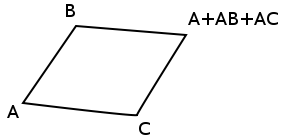
\includegraphics[scale=0.50]{images/quad.png}
	\captionof{figure}{Quadrilateral}
	\label{fig:quad}
\end{center}

\subsubsection{Box}
\indent \indent Uma caixa definida por um dos vértices desta, e 3 vectores correspondentes a cada uma das 
arestas que contém este vértice.

\cleardoublepage
\subsection{Reflection}

\begin{center}
	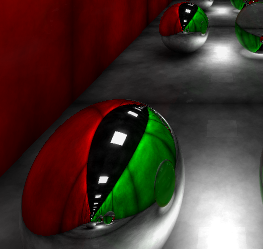
\includegraphics[scale=0.50]{images/reflection.png}
	\captionof{figure}{Reflection}
	\label{fig:reflection}
\end{center}

\indent No modelo físico a componente difusa de um material corresponde à reflecção da luz numa superfície
que contém micro-ruído. A luz ao insidir nesta superfície é espalhada para várias direcções. 

\indent Este fenómeno é facilmente reproduzido na fase de \emph{photon-mapping}.
No entanto, na fase de \emph{ray-tracing} seria necessário projectar, para cada reflecção, vários raios, o que
é computacionalmente muito exigente, pelo que para este caso é utilizada outro método.

\subsubsection{Specular}
\indent \indent Tal como indicado, caso a reflecção seja especular os raios (e fotões) obtém uma nova direcção,
calculada através da normal à superfície, e a cor provém destes. 

\subsubsection{Diffuse}
\indent Caso a reflecção seja difusa a cor é inferida a partir da radiosidade local,
isto é, pela intensidade\footnote[1]{A importância de cada fotão depende do coseno do ângulo formado entre a sua direcção e a da normal à superfície} dos fotões perto do ponto de reflecção.

\indent Um efeito visível com esta técnica é o \emph{color bleeding}: transferência de cor entre duas superfícies
através de reflecções difusas.

\cleardoublepage
\subsection{Refraction}
\begin{center}
	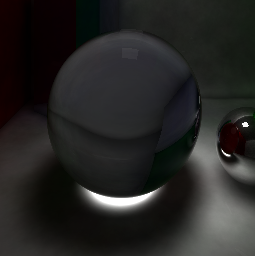
\includegraphics[scale=0.50]{images/caustics.png}
	\captionof{figure}{Caustics}
	\label{fig:caustics}
\end{center}

\indent A refracção é um efeito visível quando a luz muda entre meios com diferentes densidades.
Este efeito caracteriza-se pela diferença entre a direcção do raio incidente e a direcção do raio emergente. 
Desta forma a sua implementação adequa-se na sua totalidade ao paradigma de ray-tracing.

\subsubsection{Attenuation}
\indent \indent Ao atravessar um material translúcido, parte da energia de um fotão é absorvida. De forma análoga,
um raio ao passar pelo mesmo material obtém parte da sua cor através da cor do material.

\subsubsection{Caustics}
\indent \indent Ao sofrer sucessivas refracções, os fotões tendem a convergir, dando origem a cáusticas luminosas.
Este efeito depende apenas do \emph{photon-mapping} pelo que sem ele (i.e.: com \emph{ray-tracing} puro)
não são observáveis.

\cleardoublepage
\subsection{Anti-Alliasing}
\begin{center}
	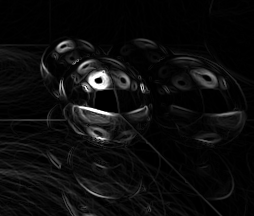
\includegraphics[scale=0.50]{images/sobel.png}
	\captionof{figure}{Sobel's operator result}
	\label{fig:sobel}
\end{center}

\indent Um método de obter melhores resultados é através da sobresamplagem da imagem (ex.: projectando
4 raios por píxel ao invés de apenas 1). No entanto este método é computacionalmente dispendioso pelo que não
deve ser aplicado à imagem na sua totalidade.

\indent Desta forma, para selecionar quais os píxeis que têm mais importância, é utilizado o operador de Sobel
para calcular a energia associada a cada pixel. Após este cálculo, apenas aqueles com energia superior a um limiar
são sobresamplados.

\cleardoublepage
\section{Gallery}
\indent \indent 

\end{document}
